% =====================================================================
% Guía del estudiante -- Geometría 8° -- Trimestre I
% María Mercedes Cantillo · Colegio San Alberto Magno
% ---------------------------------------------------------------------
% Hilo conductor: Tales de Mileto y la medición de la gran pirámide
% Plan (etapas A y B): guia-periodo-I-triangulos.plan.md
% Temas (de curriculo/programacion.csv, sesiones 003-011):
%   angulostriangulo, congruencia, semejanza, pitagoras, teoremathales
% Cada \tema tiene \label{tema:...} para que las clases lo citen con
% \refguia{tema:...}. No borrar el .aux de esta guía.
% Ejercicios: recursos/banco/matematicas/triangulos-geometria-8.py y los
% reusados (triangulos-8, pitagoras-8).
%
% Compilar:  latexmk -pdf guia-periodo-I-triangulos.tex
% =====================================================================
\documentclass[11pt]{article}
\makeatletter\def\input@path{{../../../../plantillas/estilo/}}\makeatother
\usepackage{mmcantillo}

% ======================== DATOS DE LA GUÍA ============================
\tipodocumento{Guía del estudiante}
\asignatura{Geometría}
\titulo{La sombra de la pirámide}
\grado{8°}
\periodo{I}
\hiloconductor{Tales de Mileto y la medición de la gran pirámide}
% ======================================================================
% DBA: matematicas grado 8 · DBA 6 — Identifica relaciones de congruencia y
%      semejanza entre las formas geométricas que configuran el diseño de un
%      objeto.
%      DBA 7 — Identifica regularidades y argumenta propiedades de figuras
%      geométricas a partir de teoremas y las aplica en situaciones reales.

\begin{document}

\encabezado

% ---------------------------------------------------------------------
% 1. Frase introductoria
% ---------------------------------------------------------------------
% verificado: https://it.wikisource.org/wiki/Il_Saggiatore/6 — «La filosofia è scritta in questo grandissimo libro […] Egli è scritto in lingua matematica, e i caratteri son triangoli, cerchi, ed altre figure geometriche»; Roma, Mascardi, 1623 (https://portalegalileo.museogalileo.it/egjr.asp?c=36261)
\frase{La filosofía está escrita en ese grandísimo libro que continuamente
está abierto ante nuestros ojos (digo: el universo) [\ldots] Está escrito
en lengua matemática, y sus caracteres son triángulos, círculos y otras
figuras geométricas.}
{Galileo Galilei, \emph{El ensayador} (1623), cap. 6 (trad. propia)~\cite{galileo}}

% ---------------------------------------------------------------------
% 2. Introducción
% ---------------------------------------------------------------------
\seccion{Introducción}

¿Cómo se mide la altura de un edificio sin subirse a él, o la distancia a
un barco sin navegar hasta allá? Hace veintiséis siglos, cuenta la
tradición, un sabio griego llamado Tales midió la altura de una pirámide de
Egipto con un bastón y su sombra. No usó más que triángulos: comparar
triángulos permite medir lo que no se puede tocar.

Este trimestre seguiremos a Tales. Aprenderemos las leyes de los ángulos de
un triángulo, cuándo dos triángulos son iguales (\emph{congruentes}) y
cuándo uno es una ampliación del otro (\emph{semejantes}); repetiremos el
cálculo de la pirámide; demostraremos con papel el teorema de Pitágoras, y
terminaremos con el teorema que lleva el nombre de Tales.

\textbf{Al terminar este trimestre podrás:}
\begin{itemize}
  \item calcular ángulos de un triángulo y justificar sus propiedades;
  \item argumentar la congruencia de dos triángulos con los criterios LLL,
        LAL y ALA, y reconocer triángulos semejantes con AA, LLL y LAL;
  \item calcular alturas y distancias inaccesibles con semejanza de
        triángulos, con escalas y con el teorema de Tales;
  \item demostrar el teorema de Pitágoras con material concreto y usarlo
        para hallar cualquier lado de un triángulo rectángulo.
\end{itemize}

Este trimestre trabaja dos Derechos Básicos de Aprendizaje del Ministerio de
Educación Nacional~\cite{mendba}:

\begin{dba}[Grado 8° · DBA 6]
Identifica relaciones de congruencia y semejanza entre las formas
geométricas que configuran el diseño de un objeto.
\end{dba}

\begin{dba}[Grado 8° · DBA 7]
Identifica regularidades y argumenta propiedades de figuras geométricas a
partir de teoremas y las aplica en situaciones reales.
\end{dba}

% ---------------------------------------------------------------------
% 3. Marco teórico
% ---------------------------------------------------------------------
\seccion{Marco teórico}

\subsubsection*{Un sabio de Mileto}

Tales vivió en Mileto, una ciudad griega en la costa de la actual Turquía,
aproximadamente entre el 624 y el 547 a.\,C.~\cite{mactutorthales}. No se
conserva nada escrito por él: todo lo que sabemos viene de autores que
vivieron siglos después, y los historiadores advierten que a los hombres
famosos de esa época se les atribuían descubrimientos que quizás no
hicieron. Aun así, la tradición lo presenta como el primero que no se
contentó con saber \emph{que} algo es cierto en geometría, sino que quiso
saber \emph{por qué}.

Proclo, un filósofo que escribió hacia el año 450 d.\,C. apoyándose en una
historia de la geometría hoy perdida de Eudemo (discípulo de Aristóteles),
cuenta que Tales fue el primero en afirmar que los ángulos opuestos por el
vértice son iguales y que en todo triángulo isósceles los ángulos de la
base son iguales; y que calculó la distancia de los barcos en el mar con un
método que requiere lo que hoy llamamos el criterio
ángulo-lado-ángulo~\cite{ogrady}.

\subsubsection*{La sombra de la pirámide}

La historia más famosa llega en dos versiones. Diógenes Laercio, en el
siglo III d.\,C., cita a un autor anterior, Jerónimo de Rodas:

% verificado: https://en.wikisource.org/wiki/Lives_of_the_Eminent_Philosophers/Book_I — I.27 (trad. Hicks): «Hieronymus informs us that he measured the pyramids by the shadow they cast, taking the observation at the hour when our shadow is of the same length as ourselves»
\begin{cita}{Diógenes Laercio, \emph{Vidas de los filósofos ilustres} I.27 (trad. propia)~\cite{diogenes}}
Jerónimo cuenta que midió las pirámides por su sombra, tomando la
observación a la hora en que nuestra sombra es tan larga como nosotros.
\end{cita}

Plutarco, en su \emph{Banquete de los siete sabios}, pone en boca de un
personaje otra versión, más geométrica, dirigida al propio Tales:

% verificado: https://penelope.uchicago.edu/Thayer/E/Roman/Texts/Plutarch/Moralia/Dinner_of_the_Seven*.html — Moralia 147A, trad. F. C. Babbitt (Loeb 222, 1928): «you simply set your walking-stick upright at the edge of the shadow which the pyramid cast, and, two triangles being formed by the intercepting of the sun's rays, you demonstrated that the height of the pyramid bore the same relation to the length of the stick as the one shadow to the other»
\begin{cita}{Plutarco, \emph{Banquete de los siete sabios}, \emph{Moralia} 147A (trad. propia)~\cite{plutarco}}
Simplemente pusiste tu bastón derecho en el extremo de la sombra que
proyectaba la pirámide y, formados dos triángulos por los rayos del sol,
demostraste que la altura de la pirámide guardaba con la longitud del
bastón la misma relación que una sombra con la otra.
\end{cita}

Ninguna de las dos es un testimonio de la época: fueron escritas entre seis
y ocho siglos después, y hay que tomarlas como \textbf{leyenda}. Lo que sí
es cierto es la matemática: como los rayos del sol llegan paralelos, los dos
triángulos son semejantes, y el método funciona. La pirámide más grande de
Guiza, la del faraón Keops, medía originalmente unos $146$ metros de
altura~\cite{egipto}, y su base es un cuadrado de unos $230$ metros de
lado~\cite{elgabry}.

\subsubsection*{Mil años antes de Pitágoras}

La relación $a^2 + b^2 = c^2$ no la inventó Pitágoras. La tablilla
babilónica Plimpton 322, escrita en Larsa (en el actual Irak) hacia
1820--1762 a.\,C. y guardada hoy en la Universidad de Columbia, contiene
ternas de números que la cumplen~\cite{columbia}. Pitágoras nació en Samos,
una isla a pocos kilómetros de Mileto, hacia el 570 a.\,C.; no escribió
libros, y la historia de que sacrificó bueyes al descubrir el teorema viene
de unos versos tardíos de autor incierto~\cite{huffman}. La demostración
escrita más antigua que conservamos es la de Euclides (\emph{Elementos},
I.47, hacia el 300 a.\,C.), y el nombre «teorema de Pitágoras» se lo
pusieron autores muy posteriores~\cite{euclidesI47, maor}.

El teorema se ha demostrado de muchísimas maneras. En 1876, James A.
Garfield, entonces congresista y años después presidente de Estados Unidos,
publicó en el \emph{New-England Journal of Education} una prueba con un
trapecio y tres triángulos rectángulos~\cite{garfield, ellermeyer}: en
matemáticas se puede llegar a la misma verdad por caminos diferentes.

\subsubsection*{Los dos teoremas de Tales}

Lo que en los países de habla hispana se llama «teorema de Tales» —una
recta paralela a un lado de un triángulo corta los otros dos lados en
segmentos proporcionales— aparece demostrado en los \emph{Elementos} de
Euclides (VI.2)~\cite{euclidesVI2}. En inglés, en cambio, \emph{Thales'
theorem} es otro resultado: todo ángulo inscrito en una semicircunferencia
es recto~\cite{mathworld}. Es el que Diógenes Laercio, citando a Pánfila,
atribuye a Tales cuando cuenta que fue el primero en inscribir un triángulo
rectángulo en un círculo~\cite{diogenes}. Los dos nombres honran al mismo
personaje.

\subsubsection*{De la sombra a la órbita}

Veinticinco siglos después, medir con triángulos seguía siendo cuestión de
vida o muerte. \textbf{Katherine Johnson} (1918--2020), matemática
estadounidense, entró en 1953 al laboratorio de la NACA (luego NASA) en
Langley. Calculó la trayectoria del primer vuelo espacial tripulado de
Estados Unidos (Alan Shepard, 1961) y, antes del vuelo orbital de John
Glenn en 1962, él mismo pidió que ella comprobara a mano los números del
computador. En 2015 recibió la Medalla Presidencial de la
Libertad~\cite{nasajohnson}.

% ---------------------------------------------------------------------
% 4. Temas
% ---------------------------------------------------------------------
\tema{Ángulos de un triángulo}\label{tema:angulostriangulo}

\begin{hilo}
Cuentan las fuentes que Tales viajó a Egipto. Los egipcios sabían medir
terrenos, pero Tales se hacía otra pregunta: \emph{¿por qué} los ángulos de
la base de un triángulo isósceles son iguales? Antes de medir pirámides hay
que conocer las leyes de los ángulos.
\end{hilo}

\textbf{Repaso.} En las semanas 01 y 02 clasificamos los triángulos. Por sus
lados: \emph{equilátero} (tres lados iguales), \emph{isósceles} (dos) y
\emph{escaleno} (ninguno). Por sus ángulos: \emph{acutángulo} (tres ángulos
agudos), \emph{rectángulo} (uno recto) y \emph{obtusángulo} (uno obtuso).
Recuerda también que dos ángulos opuestos por el vértice son iguales y que,
si dos rectas paralelas son cortadas por una secante, los ángulos alternos
internos son iguales.

\begin{teorema}[Suma de los ángulos internos]
En todo triángulo, los tres ángulos internos suman $180^\circ$.
\end{teorema}

\emph{Dos argumentos.} Con papel: recorta un triángulo, corta sus tres
esquinas y júntalas; forman un ángulo llano. Eso nos convence, pero no es
una demostración (¿y si el papel se dobló un poco?). La demostración usa
paralelas: por el vértice $C$ se traza la recta paralela a $AB$. Los
ángulos $\alpha'$ y $\beta'$ son alternos internos con $\alpha$ y $\beta$,
así que son iguales a ellos, y los tres ángulos en $C$ forman un ángulo
llano: $\alpha + \gamma + \beta = 180^\circ$. \hfill$\square$

\begin{center}
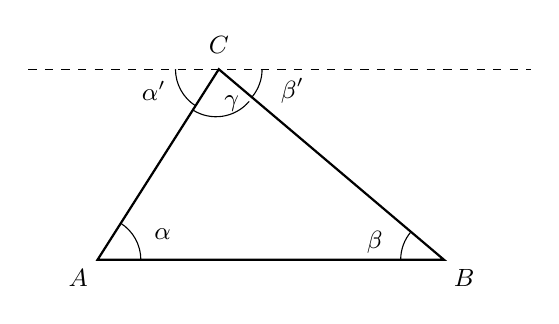
\begin{tikzpicture}[scale=1.1, every node/.style={font=\small}]
  \coordinate (A) at (0,0); \coordinate (B) at (4,0); \coordinate (C) at (1.4,2.2);
  \draw[thick] (A) -- (B) -- (C) -- cycle;
  \draw[dashed] (-0.8,2.2) -- (5,2.2);
  \node[below left] at (A) {$A$}; \node[below right] at (B) {$B$};
  \node[above=2pt] at (C) {$C$};
  \draw (0.5,0) arc (0:57.5:0.5); \node at (0.75,0.3) {$\alpha$};
  \draw (3.5,0) arc (180:139.8:0.5); \node at (3.2,0.2) {$\beta$};
  \draw (1.1,1.73) arc (237.5:319.8:0.5) ; \node at (1.55,1.8) {$\gamma$};
  \draw (0.9,2.2) arc (180:237.5:0.5); \node at (0.65,1.95) {$\alpha'$};
  \draw (1.9,2.2) arc (0:-40.2:0.5); \node at (2.25,1.95) {$\beta'$};
\end{tikzpicture}

{\small La paralela por $C$: $\alpha' = \alpha$ y $\beta' = \beta$ (alternos internos).}
\end{center}

\begin{definicion}[Ángulo externo]
Un \textbf{ángulo externo} se forma entre un lado del triángulo y la
prolongación del lado vecino. Es suplementario del ángulo interno
adyacente, y por eso es igual a la \textbf{suma de los dos ángulos
internos no adyacentes}. Los tres ángulos externos (uno en cada vértice)
suman $360^\circ$.
\end{definicion}

\textbf{Consecuencias.} Un triángulo tiene a lo sumo un ángulo recto u
obtuso; los dos ángulos agudos de un triángulo rectángulo son
complementarios; y, como sabía Tales, en un triángulo isósceles los ángulos
de la base son iguales.

% Ejercicio: triangulos-8-015
\begin{ejemplo}[Un ángulo agudo doble del otro]
Los ángulos agudos de un triángulo rectángulo son tales que uno es el doble
del otro. Como son complementarios, $x + 2x = 90^\circ$ y $x = 30^\circ$:
los tres ángulos miden $30^\circ$, $60^\circ$ y $90^\circ$.
\end{ejemplo}

\begin{aplicacion}[La cercha de un techo]
Las cerchas que sostienen los techos de muchas casas y bodegas son
triángulos isósceles. Si el carpintero conoce el ángulo del vértice de
arriba, no necesita medir los otros dos: los calcula con la suma de
ángulos, y así corta las piezas antes de subirlas.
\end{aplicacion}

\begin{preguntas}
% Ejercicio: triangulos-8-017
\pregunta El ángulo opuesto a la base de un triángulo isósceles mide
$50^\circ$. ¿Cuánto miden los otros dos ángulos internos?
\espacio{2cm}
% Ejercicio: triangulos-8-021
\pregunta En el triángulo $ABC$, el ángulo con vértice en $A$ mide
$30^\circ$ y el ángulo externo en $B$ mide $110^\circ$. ¿Cuánto mide el
ángulo $C$?
\espacio{2.5cm}
% Ejercicio: triangulos-8-014
\Needspace{8\baselineskip}
\pregunta Indica si la afirmación es verdadera o falsa y argumenta tu
respuesta: «Ningún triángulo puede tener más de un ángulo obtuso».
\espacio{2.5cm}
% Ejercicio: triangulos-8-018
\pregunta El ángulo opuesto a la base de un triángulo isósceles mide el
doble de cada uno de los otros dos. ¿Cuánto miden los ángulos internos de
ese triángulo?
\espacio{2.5cm}
\end{preguntas}

\begin{resumen}
\begin{itemize}
  \item Los ángulos internos de un triángulo suman $180^\circ$; se
        demuestra con una paralela y los ángulos alternos internos.
  \item Un ángulo externo es igual a la suma de los dos internos no
        adyacentes; los tres externos suman $360^\circ$.
  \item En un triángulo isósceles los ángulos de la base son iguales.
\end{itemize}
\end{resumen}

% ---------------------------------------------------------------------
\tema{Congruencia de triángulos}\label{tema:congruencia}

\begin{hilo}
Según Eudemo, Tales calculaba desde la costa la distancia a un barco. Si se
conocen un lado y los dos ángulos de sus extremos, el triángulo queda
determinado: se puede copiar en tierra firme y medir allí la distancia que
en el mar no se puede medir.
\end{hilo}

\begin{definicion}[Triángulos congruentes]
Dos triángulos son \textbf{congruentes} si tienen sus lados y sus ángulos
correspondientes iguales; es decir, si uno se puede llevar exactamente sobre
el otro moviéndolo (trasladándolo, girándolo o reflejándolo). Se escribe
$\triangle ABC \cong \triangle DEF$, y el orden de las letras dice qué
vértice corresponde a cuál: $A$ con $D$, $B$ con $E$ y $C$ con $F$.
\end{definicion}

No hace falta comparar los seis elementos: bastan tres bien escogidos.

\begin{teorema}[Criterios de congruencia]
Dos triángulos son congruentes si tienen iguales:
\begin{itemize}
  \item \textbf{LLL:} sus tres lados;
  \item \textbf{LAL:} dos lados y el ángulo \emph{comprendido} entre ellos;
  \item \textbf{ALA:} dos ángulos y el lado \emph{comprendido} entre ellos.
\end{itemize}
\end{teorema}

\textbf{Cuidado: con tres ángulos no basta.} Dos triángulos con los mismos
tres ángulos pueden tener distinto tamaño (piensa en un triángulo dibujado
y su fotocopia ampliada). Tampoco basta, en general, con dos lados y un
ángulo que \emph{no} esté entre ellos: con el compás se pueden construir
dos triángulos distintos con esos datos. Algunos libros dan «dos ángulos
iguales» como criterio de congruencia: es un error, porque con dos ángulos
iguales los triángulos solo son \emph{semejantes} (tema siguiente).

\begin{ejemplo}[El barco de Tales]
Desde dos puntos $A$ y $B$ de la costa se ve un barco $C$. Se miden la
distancia $AB$ y los ángulos $\angle CAB$ y $\angle CBA$. En tierra firme,
lejos del agua, se construye un triángulo $A'B'C'$ con $A'B' = AB$ y los
mismos dos ángulos. Por ALA, $\triangle A'B'C' \cong \triangle ABC$, así
que $A'C' = AC$: la distancia al barco se mide en tierra.
\end{ejemplo}

\begin{center}
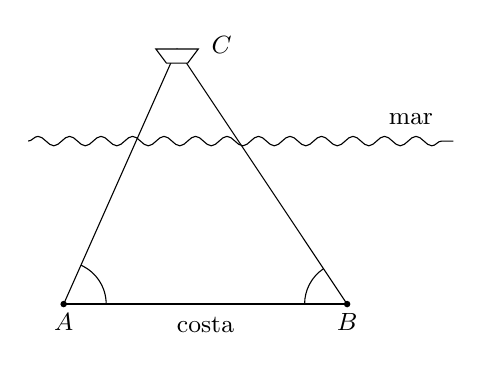
\begin{tikzpicture}[scale=0.9, every node/.style={font=\small}]
  \draw[decorate, decoration={snake, amplitude=0.6mm, segment length=4mm}]
       (-0.5,2.3) -- (5.5,2.3);
  \node[above] at (4.9,2.4) {mar};
  \coordinate (A) at (0,0); \coordinate (B) at (4,0); \coordinate (C) at (1.6,3.6);
  \draw[thick] (A) -- (B); \draw (A) -- (C) -- (B);
  \fill (A) circle (1.3pt) node[below] {$A$};
  \fill (B) circle (1.3pt) node[below] {$B$};
  \draw[fill=white] (1.3,3.6) -- (1.9,3.6) -- (1.75,3.4) -- (1.45,3.4) -- cycle;
  \node[right] at (1.95,3.65) {$C$};
  \draw (0.6,0) arc (0:66:0.6); \draw (3.4,0) arc (180:124:0.6);
  \node[below] at (2,-0.05) {costa};
\end{tikzpicture}
\end{center}

\begin{aplicacion}[La rigidez del triángulo]
Por el criterio LLL, tres barras de longitudes fijas solo forman un
triángulo, con ángulos fijos: el triángulo no se deforma. Un marco de cuatro
barras, en cambio, se aplasta. Por eso las torres de energía, los puentes
metálicos y las cerchas de los techos están hechos de triángulos.
\end{aplicacion}

\begin{preguntas}
% Ejercicio: triangulos-geometria-8-001
\pregunta En cada caso se sabe lo que se indica sobre los triángulos $ABC$
y $DEF$. ¿Qué criterio permite asegurar que son congruentes? Si ninguno,
dilo.
\begin{opciones*}(2)
  \item $AB = DE$, $BC = EF$, $CA = FD$.
  \item $AB = DE$, $\angle B = \angle E$, $BC = EF$.
  \item $\angle A = \angle D$, $AB = DE$, $\angle B = \angle E$.
  \item $\angle A = \angle D$, $\angle B = \angle E$, $\angle C = \angle F$.
\end{opciones*}
\espacio{3cm}
% Ejercicio: triangulos-geometria-8-002
\pregunta Desde dos puntos $A$ y $B$ de la playa, separados $100$~m, se ve
un barco $C$. El ángulo $\angle CAB$ mide $60^\circ$ y el ángulo
$\angle CBA$ mide $70^\circ$. Dibuja en tu cuaderno, a escala
$1$~cm $= 10$~m, un triángulo con esos datos. ¿Qué criterio asegura que tu
dibujo es una copia fiel del triángulo real? Mide en el dibujo y estima la
distancia de $A$ al barco.
\espacio{3cm}
\end{preguntas}

\begin{resumen}
\begin{itemize}
  \item Congruentes: mismos lados y mismos ángulos; uno se lleva sobre el
        otro con un movimiento. El orden de los vértices importa.
  \item Criterios: LLL, LAL (ángulo comprendido) y ALA (lado comprendido).
  \item Tres ángulos iguales \emph{no} garantizan congruencia: solo
        semejanza.
\end{itemize}
\end{resumen}

% ---------------------------------------------------------------------
\tema{Semejanza de triángulos}\label{tema:semejanza}

\begin{hilo}
Tales frente a la pirámide: no puede subir a medirla, pero sí medir su
sombra. Según Jerónimo, esperó la hora en que la sombra de una persona es
igual a su estatura; según Plutarco, comparó la sombra de la pirámide con la
de un bastón. La segunda versión funciona a cualquier hora del día. Veamos
por qué.
\end{hilo}

\begin{definicion}[Triángulos semejantes]
Dos triángulos son \textbf{semejantes} si tienen sus ángulos
correspondientes iguales y sus lados correspondientes proporcionales. El
cociente entre lados correspondientes es la \textbf{razón de semejanza}
$k$. Se escribe $\triangle ABC \sim \triangle DEF$.
\end{definicion}

\begin{teorema}[Criterios de semejanza]
Dos triángulos son semejantes si:
\begin{itemize}
  \item \textbf{AA:} tienen dos ángulos iguales (el tercero también lo
        será, porque todos suman $180^\circ$);
  \item \textbf{LLL:} sus tres lados son proporcionales;
  \item \textbf{LAL:} dos lados son proporcionales y el ángulo comprendido
        es igual.
\end{itemize}
\end{teorema}

La congruencia es el caso $k = 1$: dos triángulos congruentes son
semejantes, pero dos semejantes no tienen por qué ser congruentes. Si la
razón de semejanza es $k$, los perímetros también están en razón $k$ (y,
como curiosidad, las áreas en razón $k^2$).

% Ejercicio: triangulos-geometria-8-005
\begin{ejemplo}[La pirámide, a la manera de Plutarco]
La base de la pirámide es un cuadrado de unos $230$~m de lado, así que su
centro está a $115$~m de cada lado. Un día, la sombra sobresale $104$~m
desde el borde de la base. Un bastón de $2$~m clavado en la punta de la
sombra da una sombra de $3$~m. Los rayos del sol son paralelos, así que
forman el mismo ángulo con el suelo en los dos triángulos, y los dos tienen
un ángulo recto: por AA son semejantes. La sombra de la pirámide, medida
desde el centro de la base, es $115 + 104 = 219$~m, y
\[
  \frac{h}{219} = \frac{2}{3} \qquad\Longrightarrow\qquad h = 146 \text{ m}.
\]
\end{ejemplo}

\begin{center}
\begin{tikzpicture}[scale=1.7, every node/.style={font=\small}]
  \draw (-0.4,0) -- (4.3,0);
  \draw[thick] (-2.3*0.5+0.35,0) coordinate (P) -- (0.35+1.15*0,1.46) coordinate (V)
               -- (0.35+1.15,0) coordinate (Q);
  \coordinate (O) at (0.35,0);
  \draw[dashed] (O) -- (V) node[midway, left] {$h$};
  \coordinate (S) at ($(O)+(2.19,0)$);
  \draw[densely dotted] (V) -- (S);
  \draw[very thick] (S) -- ++(0,0.4) coordinate (T);
  \coordinate (S2) at ($(S)+(0.6,0)$);
  \draw[densely dotted] ($(T)+(-0.45,0.3)$) -- (S2);
  \node[above] at (T) {bastón};
  \draw[|<->|] ($(O)+(0,-0.15)$) -- node[below] {$115$} ($(Q)+(0,-0.15)$);
  \draw[|<->|] ($(Q)+(0,-0.15)$) -- node[below] {$104$} ($(S)+(0,-0.15)$);
  \draw[|<->|] ($(S)+(0,-0.15)$) -- node[below] {$3$} ($(S2)+(0,-0.15)$);
  \node[right] at ($(S)+(0,0.2)$) {$2$};
\end{tikzpicture}

{\small La pirámide y el bastón (medidas en metros; el dibujo no está a escala). Las líneas
punteadas son rayos de sol paralelos.}
\end{center}

\begin{aplicacion}[Planos y mapas]
Un mapa a escala $1:50\,000$ es una figura semejante a la realidad con
razón $k = \frac{1}{50\,000}$: cada centímetro del mapa representa
$50\,000$~cm, es decir, $500$~m. Por eso los ángulos del mapa son los
mismos del terreno, y los triángulos que forman tres lugares en el mapa son
semejantes a los reales.
\end{aplicacion}

\begin{preguntas}
% Ejercicio: triangulos-geometria-8-003
\pregunta ¿Son semejantes? Si lo son, di el criterio y la razón de
semejanza.
\begin{opciones*}(1)
  \item Un triángulo con ángulos de $40^\circ$ y $60^\circ$ y otro con
        ángulos de $60^\circ$ y $80^\circ$.
  \item Un triángulo de lados $4$, $6$, $8$ y otro de lados $6$, $9$, $12$.
  \item Un triángulo de lados $3$, $4$, $5$ y otro de lados $6$, $8$, $11$.
\end{opciones*}
\espacio{3cm}
% Ejercicio: triangulos-geometria-8-004
\pregunta A cierta hora de la mañana, un palo de escoba de $1{,}5$~m puesto
vertical en el patio proyecta una sombra de $2$~m. A la misma hora, la
sombra de un edificio mide $24$~m. ¿Cuánto mide el edificio? Explica por
qué los dos triángulos son semejantes.
\espacio{3cm}
\end{preguntas}

\begin{resumen}
\begin{itemize}
  \item Semejantes: mismos ángulos y lados proporcionales, con razón $k$.
  \item Criterios: AA, LLL (lados proporcionales), LAL (dos lados
        proporcionales y el ángulo comprendido igual).
  \item Con rayos de sol paralelos, un objeto y su sombra forman triángulos
        semejantes a los de cualquier otro objeto a la misma hora: así se
        mide una altura inaccesible.
\end{itemize}
\end{resumen}

% ---------------------------------------------------------------------
\tema{Teorema de Pitágoras}\label{tema:pitagoras}

\begin{hilo}
Una generación después de Tales, en la isla de Samos, a pocos kilómetros
de Mileto, crece Pitágoras. La relación que lleva su nombre ya estaba en las
tablillas babilónicas mil años antes. Lo que sí hicieron los griegos fue
\textbf{demostrarla}.
\end{hilo}

En un triángulo rectángulo, los lados que forman el ángulo recto son los
\textbf{catetos} ($a$ y $b$) y el lado opuesto al ángulo recto, el más
largo, es la \textbf{hipotenusa} ($c$).

\begin{teorema}[Teorema de Pitágoras y su recíproco]
En todo triángulo rectángulo, $a^2 + b^2 = c^2$. Y al revés: si los lados
de un triángulo cumplen $a^2 + b^2 = c^2$, el triángulo es rectángulo.
\end{teorema}

\begin{ejemplo}[Demostración con dos cuadrados]
En un cuadrado de lado $a + b$ se colocan cuatro triángulos rectángulos
iguales, de catetos $a$ y $b$ e hipotenusa $c$, como en la figura. En el
centro queda un cuadrado de lado $c$ (sus ángulos son rectos porque los dos
ángulos agudos de cada triángulo suman $90^\circ$). El área del cuadrado
grande, calculada de dos maneras:
\[
  (a + b)^2 = 4 \cdot \frac{ab}{2} + c^2
  \quad\Longrightarrow\quad a^2 + 2ab + b^2 = 2ab + c^2
  \quad\Longrightarrow\quad a^2 + b^2 = c^2.
\]
\end{ejemplo}

\begin{center}
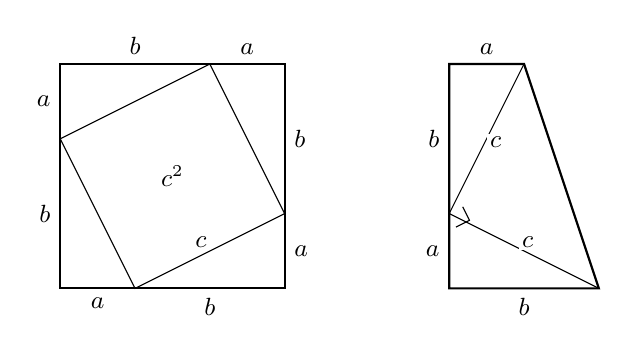
\begin{tikzpicture}[scale=0.95, every node/.style={font=\small}]
  \draw[thick] (0,0) rectangle (3,3);
  \draw (1,0) -- (3,1) -- (2,3) -- (0,2) -- cycle;
  \node[below] at (0.5,0) {$a$}; \node[below] at (2,0) {$b$};
  \node[right] at (3,0.5) {$a$}; \node[right] at (3,2) {$b$};
  \node[above] at (2.5,3) {$a$}; \node[above] at (1,3) {$b$};
  \node[left] at (0,2.5) {$a$}; \node[left] at (0,1) {$b$};
  \node at (1.5,1.5) {$c^2$};
  \node[above left, inner sep=1pt] at (2,0.5) {$c$};
  % Garfield
  \begin{scope}[xshift=5.2cm]
    \draw[thick] (0,0) -- (2,0) -- (1,3) -- (0,3) -- cycle;
    \draw (2,0) -- (0,1) -- (1,3);
    \node[below] at (1,0) {$b$}; \node[above] at (0.5,3) {$a$};
    \node[left] at (0,0.5) {$a$}; \node[left] at (0,2) {$b$};
    \node[fill=white, inner sep=1pt] at (1.05,0.62) {$c$};
    \node[fill=white, inner sep=1pt] at (0.62,1.95) {$c$};
    \draw (0.18,1.09) -- (0.27,0.91) -- (0.09,0.82);
  \end{scope}
\end{tikzpicture}

{\small Izquierda: los cuatro triángulos en el cuadrado de lado $a + b$.
Derecha: el trapecio de Garfield.}
\end{center}

\begin{ejemplo}[La prueba de Garfield]
El trapecio de la derecha tiene bases $a$ y $b$ y altura $a + b$, y está
formado por dos triángulos rectángulos de catetos $a$ y $b$ y un triángulo
rectángulo isósceles de catetos $c$. Igualando áreas,
\[
  \frac{(a + b)(a + b)}{2} = 2 \cdot \frac{ab}{2} + \frac{c^2}{2};
\]
al multiplicar por $2$ queda $a^2 + 2ab + b^2 = 2ab + c^2$, es decir,
$a^2 + b^2 = c^2$. Es media figura de la demostración anterior.
\end{ejemplo}

Con el teorema se halla cualquier lado de un triángulo rectángulo:
$c = \sqrt{a^2 + b^2}$ para la hipotenusa y $a = \sqrt{c^2 - b^2}$ para un
cateto. Las \textbf{ternas pitagóricas} son tríos de enteros que cumplen la
relación, como $3, 4, 5$ o $5, 12, 13$: la tablilla Plimpton 322 es la
tabla de ternas más antigua que conocemos.

\begin{aplicacion}[La escuadra del maestro de obra]
Para comprobar que la esquina de una construcción es recta, los maestros de
obra marcan $60$~cm sobre un muro y $80$~cm sobre el otro, y verifican que
entre las marcas haya exactamente $1$~m: es la terna $3, 4, 5$ multiplicada
por $20$. Por el recíproco del teorema, si la medida da, la esquina es
recta.
\end{aplicacion}

\begin{preguntas}
% Ejercicio: pitagoras-8-008, pitagoras-8-005
\pregunta ¿Pueden ser los lados de un triángulo rectángulo (el mayor es la
hipotenusa)? Justifica con el recíproco del teorema.
\begin{opciones*}(2)
  \item $21$, $20$ y $29$
  \item $12$, $16$ y $20$
\end{opciones*}
\espacio{2.5cm}
% Ejercicio: pitagoras-8-036, pitagoras-8-026
\pregunta En un triángulo rectángulo:
\begin{opciones*}(1)
  \item los catetos miden $12$ y $5$. Halla la hipotenusa.
  \item un cateto mide $7$ y la hipotenusa mide $\sqrt{53}$. Halla el otro
        cateto.
\end{opciones*}
\espacio{2.5cm}
% Ejercicio: triangulos-geometria-8-006
\pregunta Para comprobar que la esquina de un muro es recta, un maestro de
obra marca $60$~cm sobre un muro y $80$~cm sobre el otro, desde la esquina,
y mide la distancia entre las dos marcas.
\begin{opciones*}(1)
  \item ¿Cuánto debe medir si la esquina es recta?
  \item Si mide $98$~cm, ¿el ángulo es mayor o menor que $90^\circ$? Explica.
\end{opciones*}
\espacio{3cm}
% Ejercicio: pitagoras-8-041
\Needspace{6\baselineskip}
\pregunta En un triángulo rectángulo un cateto mide $6$ y la hipotenusa
mide $6\sqrt{2}$. Halla la longitud del otro cateto.
\espacio{2.5cm}
\end{preguntas}

\begin{resumen}
\begin{itemize}
  \item En un triángulo rectángulo, $a^2 + b^2 = c^2$ ($c$: hipotenusa); y
        si $a^2 + b^2 = c^2$, el triángulo es rectángulo.
  \item Se demuestra comparando áreas: cuatro triángulos en un cuadrado de
        lado $a + b$, o el trapecio de Garfield.
  \item Hipotenusa: $c = \sqrt{a^2 + b^2}$; cateto: $a = \sqrt{c^2 - b^2}$.
\end{itemize}
\end{resumen}

% ---------------------------------------------------------------------
\tema{Teorema de Thales}\label{tema:teoremathales}

\begin{hilo}
Volvamos a la sombra de la pirámide. Lo que Tales usó no era un truco para
un día de sol, sino una ley general de las rectas paralelas. Euclides la
escribió unos dos siglos y medio después; hoy lleva el nombre de Tales.
\end{hilo}

\begin{teorema}[Teorema de Tales]
Si una recta paralela a un lado de un triángulo corta los otros dos lados,
los divide en segmentos proporcionales: si $DE \parallel BC$, entonces
\[
  \frac{AD}{DB} = \frac{AE}{EC}.
\]
Y al revés (recíproco): si los segmentos son proporcionales, la recta $DE$
es paralela a $BC$. Lo mismo vale para dos rectas cualesquiera cortadas por
varias paralelas.
\end{teorema}

\begin{center}
\begin{tikzpicture}[scale=1.1, every node/.style={font=\small}]
  \coordinate (A) at (1.5,3); \coordinate (B) at (0,0); \coordinate (C) at (4,0);
  \coordinate (D) at ($(A)!0.4!(B)$); \coordinate (E) at ($(A)!0.4!(C)$);
  \draw[thick] (A) -- (B) -- (C) -- cycle;
  \draw[dashed] (D) -- (E);
  \node[above] at (A) {$A$}; \node[below left] at (B) {$B$};
  \node[below right] at (C) {$C$}; \node[left] at (D) {$D$};
  \node[right] at (E) {$E$};
  \fill (D) circle (1.2pt); \fill (E) circle (1.2pt);
\end{tikzpicture}

{\small $DE \parallel BC$: el triángulo $ADE$ es semejante al triángulo $ABC$.}
\end{center}

La razón es la del tema 3: los triángulos $ADE$ y $ABC$ comparten el ángulo
$A$ y tienen los ángulos en $D$ y en $B$ iguales (correspondientes entre
paralelas), así que son semejantes por AA. En la pirámide, el rayo de sol
que pasa por la punta del bastón es paralelo al que pasa por la cima.

\begin{ejemplo}[Dividir un segmento sin medirlo]
Para partir un segmento $AB$ en tres partes iguales, se traza desde $A$ una
semirrecta auxiliar y se marcan en ella con el compás tres segmentos
iguales, $AP_1 = P_1P_2 = P_2P_3$. Se une $P_3$ con $B$ y por $P_1$ y $P_2$
se trazan paralelas a $P_3B$. Por el teorema de Tales, las paralelas cortan
$AB$ en segmentos proporcionales a los de la semirrecta, que son iguales:
$AB$ queda dividido en tres partes iguales.
\end{ejemplo}

En GeoGebra puedes construir la figura del teorema, mover los puntos y
comprobar que las razones $\frac{AD}{DB}$ y $\frac{AE}{EC}$ siguen siendo
iguales.

\textbf{El otro teorema de Tales.} En los libros en inglés, \emph{Thales'
theorem} es este: si $AB$ es un diámetro de una circunferencia y $C$ es
cualquier otro punto de ella, el ángulo $ACB$ es recto.

\begin{aplicacion}[Franjas iguales sin regla graduada]
Las líneas de un cuaderno son paralelas y equidistantes. Si pones una tira
de papel inclinada sobre ellas, las líneas la cortan en partes iguales, sea
cual sea su largo: es el teorema de Tales. Así se divide una cartulina en
franjas iguales sin hacer cuentas.
\end{aplicacion}

\begin{preguntas}
% Ejercicio: triangulos-geometria-8-007
\pregunta En el triángulo $ABC$, $DE \parallel BC$ ($D$ en $AB$, $E$ en
$AC$). Si $AD = 4$, $DB = 6$ y $AE = 5$, halla $EC$ y $AC$.
\espacio{2cm}
% Ejercicio: triangulos-geometria-8-008
\pregunta En el triángulo $ABC$ se marcan $D$ en $AB$ y $E$ en $AC$. ¿Es
$DE$ paralela a $BC$? Justifica con el recíproco del teorema de Tales.
\begin{opciones*}(1)
  \item $AD = 3$, $DB = 4{,}5$, $AE = 4$, $EC = 6$.
  \item $AD = 3$, $DB = 4{,}5$, $AE = 4$, $EC = 5$.
\end{opciones*}
\espacio{2.5cm}
\end{preguntas}

\begin{resumen}
\begin{itemize}
  \item Teorema de Tales: una paralela a un lado de un triángulo corta los
        otros dos en segmentos proporcionales; y si son proporcionales, la
        recta es paralela.
  \item Es la semejanza del tema 3 vista de otra manera: el triángulo
        pequeño y el grande son semejantes por AA.
  \item Con paralelas se divide un segmento en partes iguales sin medirlo.
\end{itemize}
\end{resumen}

% ---------------------------------------------------------------------
% 5. Cierre del hilo conductor
% ---------------------------------------------------------------------
\seccion{Cierre: medir sin tocar}

De la sombra de un bastón a la trayectoria de una cápsula espacial: Tales
—según la leyenda— midió una pirámide comparando triángulos; Pitágoras y
Euclides demostraron relaciones que los babilonios ya usaban, y Katherine
Johnson, veinticinco siglos después, confió vidas humanas a la misma
geometría. La lección del trimestre: la congruencia copia, la semejanza
agranda y achica, y los teoremas permiten medir sin tocar. Y otra lección:
de Tales sabemos poco y se cuenta mucho, pero sus triángulos cualquiera los
puede dibujar y comprobar. En el trimestre siguiente pasaremos de las
figuras planas a los sólidos: el volumen de prismas y otros cuerpos.

% ---------------------------------------------------------------------
% 6. Evaluación (secciones institucionales)
% ---------------------------------------------------------------------
\matrizevaluacion
  {Enuncia la suma de ángulos del triángulo, los criterios de congruencia y
   de semejanza y los teoremas de Pitágoras y de Tales; distingue congruente
   de semejante.}
  {Justifica congruencias y semejanzas con el criterio adecuado; demuestra el
   teorema de Pitágoras con material concreto; calcula lados, alturas y
   distancias inaccesibles con semejanza, Pitágoras y Tales.}
  {Argumenta sus respuestas con criterios y no con «se ve igual»; revisa sus
   medidas y cálculos.}
  {Trabaja en equipo en las mediciones con sombras y en las construcciones;
   distingue lo demostrado de lo que se cuenta como leyenda.}

\autoevaluacion

\seguimientodocente

% ---------------------------------------------------------------------
% 7. Referencias
% ---------------------------------------------------------------------
\begin{referencias}
% verificado: https://exhibitions.library.columbia.edu/exhibits/show/plimpton/mathematics/page-2 — Plimpton 322: Larsa, ca. 1820–1762 a. C., ternas pitagóricas; Rare Book & Manuscript Library
\bibitem{columbia} Columbia University Libraries. \emph{«Our Tools of
  Learning»: George Arthur Plimpton's Gifts to Columbia University}
  (exhibición en línea), Plimpton 322. Nueva York: Columbia University.
% verificado: https://en.wikisource.org/wiki/Lives_of_the_Eminent_Philosophers/Book_I — I.24 (Pánfila: triángulo rectángulo inscrito en el círculo) y I.27 (Jerónimo: la sombra); edición Loeb 184 en https://www.hup.harvard.edu/books/9780674992030
\bibitem{diogenes} Diógenes Laercio (1925). \emph{Lives of Eminent
  Philosophers}, vol. I (trad. R. D. Hicks; Loeb Classical Library, 184).
  Cambridge, MA: Harvard University Press. Libro I, 24 y 27.
% verificado: https://egymonuments.gov.eg/en/monuments/the-great-pyramid — «with its original height of 146.5 meters»
\bibitem{egipto} Ministry of Tourism and Antiquities (Egipto). \emph{The
  Great Pyramid}. \url{https://egymonuments.gov.eg}
% verificado: https://pmc.ncbi.nlm.nih.gov/articles/PMC13194686/ — «base length of approximately 230.33 m per side»; «originally constructed to a height of 146.59 m»
\bibitem{elgabry} ElGabry, M., Hamed, A., Yoshimura, S., Hussein, H. M.,
  Maklad, M. y Salama, A. (2026). Architectural and geotechnical aspects
  affecting earthquake resilience for the antique Egyptian Khufu pyramid.
  \emph{Scientific Reports}.
% verificado: https://facultyweb.kennesaw.edu/sellerme/docs/garfieldpro.pdf — Garfield, 1876, prueba con un trapecio
\bibitem{ellermeyer} Ellermeyer, S. F. \emph{James Garfield's Proof of the
  Pythagorean Theorem}. Kennesaw State University.
% verificado: https://mathcs.clarku.edu/~djoyce/elements/bookI/propI47.html — I.47; el nombre lo dieron Proclo y otros siglos después; conocido por los babilonios más de mil años antes
\bibitem{euclidesI47} Euclides (ca. 300 a.\,C.). \emph{Elementos}, Libro I,
  proposición 47 (edición electrónica de D. E. Joyce, Clark University).
% verificado: https://mathcs.clarku.edu/~djoyce/elements/bookVI/propVI2.html — VI.2: una paralela a un lado corta los otros dos proporcionalmente, y su recíproco
\bibitem{euclidesVI2} Euclides (ca. 300 a.\,C.). \emph{Elementos}, Libro VI,
  proposición 2 (edición electrónica de D. E. Joyce, Clark University).
% verificado: https://www.jstor.org/stable/44764657 — «Pons Asinorum», J. A. G., New England Journal of Education 3(14), 1 abr. 1876, p. 161 (registro de JSTOR por búsqueda; la página no cargó el texto)
\bibitem{garfield} Garfield, J. A. (1876, 1 de abril). Pons asinorum.
  \emph{New-England Journal of Education}, 3(14), 161.
% verificado: https://it.wikisource.org/wiki/Il_Saggiatore/6 — texto italiano, cap. 6; Roma, Giacomo Mascardi, 1623 (https://portalegalileo.museogalileo.it/egjr.asp?c=36261)
\bibitem{galileo} Galilei, G. (1623). \emph{Il Saggiatore}. Roma: Giacomo
  Mascardi.
% verificado: https://plato.stanford.edu/entries/pythagoras/ — rev. 5 feb. 2024; ca. 570–490 a. C., no escribió libros, versos del sacrificio de autor incierto
\bibitem{huffman} Huffman, C. (2024). Pythagoras. En E. N. Zalta y
  U. Nodelman (eds.), \emph{Stanford Encyclopedia of Philosophy}.
% verificado: https://mathshistory.st-andrews.ac.uk/Biographies/Thales/ — ca. 624–547 a. C.; relatos de la pirámide; advertencia sobre atribuciones
\bibitem{mactutorthales} O'Connor, J. J. y Robertson, E. F. \emph{Thales of
  Miletus}. MacTutor History of Mathematics, Universidad de St Andrews.
% verificado: https://www.jstor.org/stable/j.ctvh9w0ks — Princeton University Press, 2007, ISBN 978-0-691-12526-8
\bibitem{maor} Maor, E. (2007). \emph{The Pythagorean Theorem: A 4,000-Year
  History}. Princeton, NJ: Princeton University Press.
% verificado: https://mathworld.wolfram.com/ThalesTheorem.html — en inglés, Thales' theorem = ángulo inscrito en una semicircunferencia es recto
\bibitem{mathworld} Weisstein, E. W. \emph{Thales' Theorem}. MathWorld,
  Wolfram Research.
% verificado: https://gblumen.mineducacion.gov.co/cgi-bin/koha/opac-detail.pl?biblionumber=4785 — MEN 2016, ISBN 978-958-691-913-5
\bibitem{mendba} Ministerio de Educación Nacional (2016). \emph{Derechos
  Básicos de Aprendizaje V.2: Matemáticas}. Bogotá: MEN.
% verificado: https://www.nasa.gov/centers-and-facilities/langley/katherine-johnson-biography/ — 1918–2020; NACA 1953; Shepard 1961; Glenn 1962; Medalla Presidencial de la Libertad 2015
\bibitem{nasajohnson} NASA. \emph{Katherine Johnson Biography}. Langley
  Research Center.
% verificado: https://iep.utm.edu/thales/ — Proclo/Eudemo: opuestos por el vértice, isósceles, distancia de los barcos (Euclides I.26)
\bibitem{ogrady} O'Grady, P. Thales of Miletus. \emph{Internet Encyclopedia
  of Philosophy}.
% verificado: https://penelope.uchicago.edu/Thayer/E/Roman/Texts/Plutarch/Moralia/Dinner_of_the_Seven*.html — Moralia 147A, Loeb Classical Library 222 (1928), trad. F. C. Babbitt
\bibitem{plutarco} Plutarco (1928). Banquete de los siete sabios. En
  \emph{Moralia}, vol. II (trad. F. C. Babbitt; Loeb Classical Library,
  222), 147A. Cambridge, MA: Harvard University Press.
\end{referencias}

\end{document}
